\documentclass{article}

\usepackage[ngerman]{babel}
\usepackage[utf8]{inputenc}
\usepackage[T1]{fontenc}
\usepackage{hyperref}
\usepackage{csquotes}
\usepackage[a4paper]{geometry}
\usepackage{graphicx}
\usepackage{float}
\usepackage{caption}
\usepackage[
    backend=biber,
    style=apa,
    sortlocale=de_DE,
    natbib=true,
    url=false,
    doi=false,
    sortcites=true,
    sorting=nyt,
    isbn=false,
    hyperref=true,
    backref=false,
    giveninits=false,
    eprint=false]{biblatex}
\addbibresource{../references/bibliography.bib}
%\parindet=0em

\title{Ethik im Umgang mit Daten}
\author{Aylina Ospina Cruz}
\date{31.05.2024}


\begin{document}

\maketitle

\abstract{
    Inwiefern beeinflusst von KI erstellte personalisierte Webung das kaufverhalten der Menschen?
    Algorithmen und Datenanalyse: KI-Algorithmen analysieren das Verhalten und die Vorlieben von Nutzern, um personalisierte Produktempfehlungen zu geben. Beispiele sind Amazon und Netflix, die personalisierte Kauf- und Sehempfehlungen basierend auf bisherigen Käufen und angesehenen Inhalten bieten. Ist es ehtisch korrekt, die Daten der Nutzer für personalisierte Werbung zu nutzen?
}


\tableofcontents


\section{Künstliche Intelligenz}

Die künstliche Intelligenz ermöglicht Maschinen und Compute,  Aufgaben zu erledigen, die eigentlich menschliche Intelligenz erfordern. Dies ist möglich, in dem man grosse Mengen an Daten sammelt und analysiert. Die Daten müssen ausserdem bereinigt werden, damit keine Falschinformationen enthalten sind. Die KI ist nicht imstande, zwischen richtigen und falschen Informationen zu unterscheiden, was zu falschen Aussagen führen kann. Diese werden dann nach wiederkehrenden Mustern abgesucht damit so Modelle erstellt werden können. Die künstliche Intelligenz wird danach mit diesen Daten trainiert und ist so imstande, Sachen wahrzunemen und zu entscheiden. Eine KI wird trainiert, indem sie mit Daten gefüttert wird, die es ihr ermöglichen, Muster zu erkennen und Vorhersagen zu treffen. Durch kontinuierliches Lernen und Anpassen der Parametern kann die KI ihre Fähigkeiten verbessern. Parameter sind die veränderlichen Werte innerhalb eines Modells. Diese Werte bestimmen, wie das Modell Eingabedaten verarbeitet und Entscheidungen trifft. Durch das Anpassen dieser Parameter lernt das Modell, Muster und Zusammenhänge in den Daten zu erkennen, um genaue Vorhersagen oder Klassifikationen zu ermöglichen. Sie wird immer wieder korrigiert und optimiert ihre Antworten. Die künstliche Intelligenz wird in Bereichen genutz: von der Automatisierung in Fertigung und Kundenservice über personalisierte Werbung und Empfehlungen bis hin zu Sprach- und Bilderkennung. Sie unterstützt auch in der Medizin, bei autonomen Systemen wie selbstfahrenden Autos, in der Finanzbranche, im Bildungswesen und in der Robotik. KI schafft neue Möglichkeiten und verbessert Effizienz und Genauigkeit in verschiedenen Bereichen.

\section{Personalisierte Werbung}
 Die Werbung unterscheidet sich von Person zu Person. Es werden passgenaue Anzeigen erstellt, die die Vorlieben, Interessen und Kaufverhalten beachten und so angepasste, personalisierte Werbung zuscheidet. Dies ist nur Möglich, wenn die Daten der Käufer gesammelt und anayilisert werden. Diese Daten stammen aus verschiedenen Quellen wie Suchhistorien, Kaufverhalten, sozialen Medien und Webseitenbesuchen. Somit ist es Möglich, Werbung genauen Zielgruppen zu zeigen und so hat man eine viel grössere Erfolgquote. Die Firmen können genau definieren, wen sie erreichen wollen und können auch verschiedene Werbung erstellen, die einige Menschen mehr anspricht wie andere. Um personalisierte Werbung zu ermöglichen, werden häufig Tracking-Technologien wie Cookies eingesetzt. Diese helfen, unser Online-Verhalten zu verfolgen und Informationen über unsere Präferenzen und Vorlieben zu sammeln. Ein Beispiel für personalisierte Werbung wäre ein Kunde, der bei einem Online-Elektronikhändler nach einem Laptop sucht. Er hat bis jetzt noch nichts gekauft. Basierend auf seinem Suchverhalten und anderen Daten, zeigt ihm der Online-Elektronikhshop Anzeigen für ähnliche Laptops und Zubehör. Ausserdem kann der Online-Shop Rabatte und Aktionen erstellen, welche den Käufer zusätzlich motivieren, das Produkt zu kaufen. Durch die kontinuierliche Anpassung der Anzeigen auf Grundlage seines Verhalten steigt die Wahrscheindlichkeit eines Klicks und Kaufs.

 \section{KI in der personalisierten Werbung}

 Die künstliche Intelligenz spielt eine grosse Rolle für die personalisierte Werbung. Sie funktioniert mithilfe von Machine Learning-Algorithmen, die den passenden Zeitpunkt und die passende Plattform für die Werbekampagne bestimmt. Machine Learning-Algorithmen sind darauf trainiert, Muster in grossen Beständen historischer Daten zu finden und auf Basis dieser Erkenntnissen und Kommentaren, Vorhersagen zu treffen. Die historischen Daten sind die Daten, die die KI im Laufe der Zeit gesammelt hat.
 Künstliche Intelligenz spielt eine entscheidende Rolle in der personalisierten Werbung, indem sie riesige Datenmengen analysiert, um das Verhalten von Verbrauchern zu verstehen und präzise Vorhersagen über deren Interessen und Bedürfnisse zu treffen. Durch maschinelles Lernen kann KI individuelle Nutzerprofile erstellen und automatisch massgeschneiderte Werbeinhalte erstellen, die auf demografischen Merkmalen, Verhaltensdaten und sogar emotionalen Signalen basieren. Diese personalisierten Anzeigen erhöhen die Relevanz für den Verbraucher und verbessern somit die Werbeeffektivität, indem sie die Wahrscheinlichkeit erhöhen, dass Nutzer auf die Anzeigen reagieren oder konvertieren. Letztendlich ermöglicht es KI den Unternehmen, ihre Marketingbudgets effizienter einzusetzen, indem sie die richtigen Botschaften zur richtigen Zeit und auf der richtigen Platform an die richtigen Personen senden.

 \begin{figure}[ht]
    \centering
    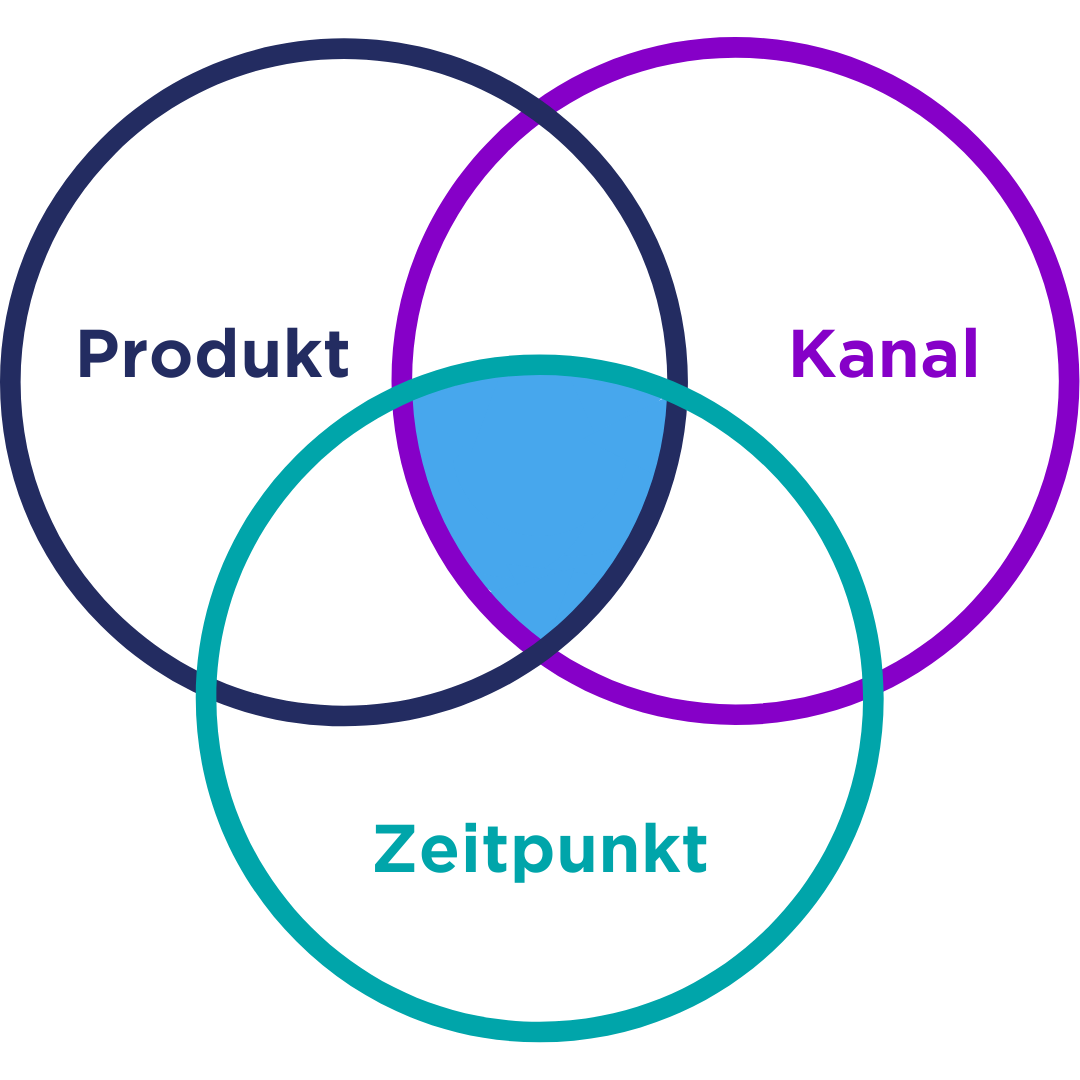
\includegraphics[width=0.3\textwidth]{Infografik.jpg}
    \caption{personalisierte Werbung}
    \label{fig:personaliserte Werbung}
    \end{figure}

 \section{Einfluss auf das Kaufverhalten}
Da die Werbung auf die Wünsche und Vorlieben der Menschen eingehen und sich vortlaufend anpassen kann, wird perfekt zugeschnitte Werbung angezeigt. Das hat einen erheblichen Einfluss auf ihr Kaufverhalten, da die Anzeigen für die Konsumenten relevanter und ansprechender ist. Der Käufer fühlt sich eher angesprochen und die Wahrscheindlichkeit steigt, dass sie auf die Werbung reagieren und ein Kauf tätigen. Ausserdem kann personalisierte Werbung das Vertrauen, das ein Kunde in eine Marke hat, stärken. Wenn Verbraucher das Gefühl haben, dass eine Marke ihre Bedürfnisse und Vorlieben versteht und ihnen relevante Produkte oder Dienstleistungen anbietet, fühlen sie sich wertgeschätzt und respektiert. Das Vertrauen, was durch diese Art von Werbung aufgebaut wird, führt oft zu Markentreue, was wiederum viel Umsatz für Firmen bedeutet. Kunden entscheiden sich lieber für Firmen und Marken, die sie als vertraueswürdig und relevant empfinden. 

\section{Problematiken bei personalisierten Werbung}

Der richtige Umgang mit den Daten der Käufer ist sehr wichtig. Die persönlichen Daten sind sehr privat und können dem Nutzer einem extrem realitätsnahen Personenprofil zuordenen. Es kann vorkommen, das die KI besser über eine Person informiert ist, als sehr nahestehenden Personen. Mit diesen Informationen hat die künstliche Inteligenz aber auch Macht. Sie kann den Nutzer gezielt manipulieren und so Sachen verkaufen. Zum Beispiel kann die KI schnell herausfinden, ob die Person Gewicht verlieren will und kann ihm so Produkte zum abnehmen presentieren. Die Wahrscheindlichkeit, dass die Person dieses Produkt kauft, obwohl er es nicht benötigt und nicht geplant hatte, dieses zu kaufen, ist extrem hoch. Somit ist ein eine gute Chance für solche Firmen, ihre Produkte verkaufen zu können. Online-Datenschutz ist sehr wichtig. Die Nutzer müssen informiert sein und sich den preisgegebenen Daten bewusst sein. Dies ist unter anderem mit dem akkzeptieren der Cookies und der Nutzungsbedingungen möglich. In einer Studie fand man heraus, dass die meisten Inernet-Nutzer personalisiertes Marketing als unethisch, mysteriös, verwirrend und sogar als unheimlich empfinden. Sie fühlen sich wertlos, da sie wie ein Objekt behandelt werden. Zudem haben viele das Gefühl, keine Kontrolle über ihre eigenen Daten zu haben und fürchten, dass diese missbraucht werden. Leider gehen zu viele Menschen zu leichtfertig mit ihren persönlichen Daten um. Darum ist der Datenschutz sehr wichtig. 
Personalisierte Werbung ist gut, wenn die Daten der Nutzer in einer sinnvollen, ethischen Weise genutzt werden. Es ist wichtig, dass am Schluss der Nutzer profitieren kann. Ausserdem sollen nur die Daten gesammelt werden, die wirklich für den Kunden zum Vorteil sind. 

Diese Informationen kommen von \citep{Basicthinking}. 

\printbibliography

\nocite{*}

\end{document}
